\Chapter{Koncepció}

\Section{Alpha-algoritmus} 

Az Alpha algoritmus (vagy Alpha bányász) mint folyamatelemzési algoritmus célja, hogy eseménysorozatok halmazából egy ok-okozat rendszert építsen fel. Először van der Aalst, Weijters és Măruşter hozta be a köztudatba. A működésében az eseménysorok halmazát nevezhetjük eseménynaplónak is. Ez az eseménynapló úgynevezett trace hal\hyp{}mazoknak a halmaza, egy trace pedig adott tevékenységnek a sorozata.

Az Alpha bányász volt a legelső folyamatbányászati módszer amit valaha javasoltak és egy egész jó rálátást biztosít a folyamatbányászat céljára, valamint arra, hogy a folyamatokban lévő különböző tevékenységek hogyan is vannak végrehajtva. Emelett, az Alpha bányász szolgált számos újabb folyamatbányászati technika (pl.: Heurisztikus bányász, genetikus bányászat) alapjaként.
	
\begin{definition}{\textit{(Munkafolyamati trace)}} Egy string a $T$ ábécé feladatai közül.\end{definition}
\begin{definition}{\textit{(Munkafolyamati napló)}} Munkafolyamati tracek halmaza.\end{definition}

\subsection{Rövid leírása}	

Az algoritmus egy munkafolyamati naplót $W \subseteq  T^*$ kap bemenetként, és eredményként egy munkafolyamati hálót épít fel.

Ezt az alapján csinálja meg, hogy megvizsgálja az általános kapcsolatokat az egyes feladatok között. Például egy adott feladat lehet, hogy minden esetben megelőz egy másik feladatot, ami egy hasznos információ.

\subsection{Eseménynapló}
Az eseménynapló az elsődleges szükséglet bármely folyamatbányászati algoritmus alkal\hyp{}mazásához. Az eseménynapló a következőket tartalmazza: egyedi azonosító az esethez, tevékenység megnevezése valamint egy időbélyeg. Egy eseménynaplót akár tevékenysé\hyp{}gek halmazának halmazaként is lehet ábrázolni.

Az Alpha bányász szabályai szerint az egyes tevékenységek között az alábbi 4 féle kapcsolat egyike lehetséges:
\begin{enumerate}
\item \textbf{Közvetlen sorrend: $x > y$} akkor és csakis akkor ha az $x$ eseményt közvetlenül követi $y$.
\item \textbf{Okozat: $x \rightarrow y$} ha $x > y$ és nem $y > x$.
\item \textbf{Párhuzam: $x \parallel y$} ha $x > y$ és $y > x$.
\item \textbf{Választás: $x \# y$} ha nem $(x > y)$ és nem $(y > x)$.
\end{enumerate}

\subsection{Minták}

\begin{figure}[h!]
\begin{center}
\caption{\textbf{Szekvencia: A $\rightarrow$ B}}

\includegraphics[width=8truecm, height=4truecm]{images/img_alpha_seq}\\
\label{fig:example}
\end{center}
\end{figure}

\begin{figure}[h!]
\begin{center}
\caption{\textbf{XOR-elágazás: A $\rightarrow$ B, A $\rightarrow$ C} és \textbf{B \# C}}
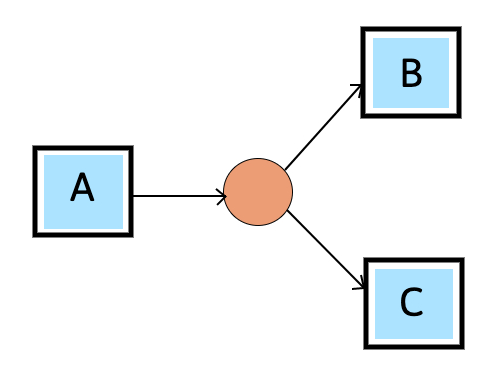
\includegraphics[width=8truecm, height=6truecm]{images/img_alpha_xor}\\
\label{fig:example}
\end{center}
\end{figure}

\begin{figure}[h!]
\begin{center}
\caption{\textbf{ÉS-elágazás: A $\rightarrow$ B, A $\rightarrow$ C} és \textbf{B $\parallel$ C}}
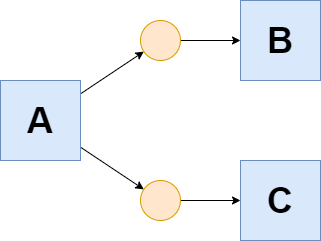
\includegraphics[width=8truecm, height=6truecm]{images/img_alpha_and}\\
\label{fig:example}
\end{center}
\end{figure}

\newpage

\subsection{Példa}
Vegyük példának a következő eseménynaplót:\\
\begin{figure}[h]
\begin{center}
\caption{Példa eseménynaplpó}
\begin{tabular}{||c | c | c ||}
	\hline
	ID & Tevékenység & Időbélyeg \\ [0.5ex]
	\hline\hline
	1 & A & 2022-10-05 13:50:40.000 \\
	\hline
	1 & B & 2022-10-05 16:30:12.000 \\
	\hline
	1 & C & 2022-10-05 16:57:31.000 \\
	\hline
	1 & D & 2022-10-06 13:50:41.000 \\
	\hline
	2 & A & 2022-10-06 15:30:27.000 \\
	\hline
	2 & C & 2022-10-06 16:23:33.000 \\
	\hline
	2 & B & 2022-10-07 08:33:02.000 \\
	\hline
	2 & D & 2022-10-07 12:41:11.000 \\
	\hline
	3 & A & 2022-10-07 13:02:57.000 \\
	\hline
	3 & E & 2022-10-07 14:11:21.000 \\
	\hline
	3 & D & 2022-10-07 14:59:22.000 \\
	\hline
\end{tabular}
\label{fig:example}
\end{center}
\end{figure}\\	
Ebben az esetben az eseménynaplót az alábbi módon tudjuk jelölni:
\[ 
	L_1 = [< A,B,C,D >, <A,C,B,D>, <A,E,D>]
\]

Az Alpha bányász úgy kezdi a munkát, hogy az eseménynaplót közvetlen-sorrend, okozat, párhuzam és választás relációkra alakítja és ezeket felhasználva létrehoz egy petri hálót ami leírja a folyamat modellét.

Első lépésként létrehoz egy lenyomati mátrixot:

\begin{figure}[h!]
\begin{center}
\caption{Példa lenyomati mátrix}
\begin{tabular}{|c | c | c | c | c | c|}
	\hline
	\hspace{0.1cm} & A & B & C & D & E \\
	\hline
	A & \# & $\rightarrow$ & $\rightarrow$ & \# & $\rightarrow$ \\
	\hline
	B & $\leftarrow$ & \# & $\parallel$ & $\rightarrow$ & \# \\
	\hline
	C & $\leftarrow$ & $\parallel$ & \# & $\rightarrow$ & \# \\
	\hline
	D  & \# & $\leftarrow$ & $\leftarrow$ & \# & $\leftarrow$ \\
	\hline
	E & $\leftarrow$ & \# & \# & $\rightarrow$ & \# \\
	\hline
\end{tabular}
\label{fig:example}
\end{center}
\end{figure}

\newpage

\noindent $Y_W$ az összes $(A,B)$  pár halmaza a feladatok maximális halmazából úgy, hogy:
\begin{itemize}
	\item {Egyik $A \times A$ és $B \times B$ sem tagja $>$-nek, és}
	\item {$A \times B$ részhalmaza $\rightarrow$-nek.}
\end{itemize}
\noindent $P_W$ tartalmazza az egyes $Y_W$-hez tartozó helyeket $p_{(A,B)}$, plussz a beviteli $i_W$ helyet és a kimeneti $o_W$ helyet.
\noindent A folyamati reláció $F_W$ az alábbiak uniójából áll össze:
\begin{itemize}
\item $\{(a,p_{(C,B)})|(A,B) \in Y_W \wedge a \in A\}$
\item $\{(p_{(A,B)},b)|(A,B) \in Y_W \wedge b \in B\}$
\item $\{(i_W,t)|t \in T_1\}$
\item $\{(t,i_0)|t \in T_0\}$
\end{itemize}

\noindent Az eredmény

\begin{itemize}
\item egy Petri háló struktúra $\alpha (W) = (P_W, T_W, F_W)$
\item egy beviteli hellyel $i_W$ és egy kimeneti hellyel $o_W$
\item mivel minden $T_W$ átmenet $F_W$-úton van $i_W$-ből $o_W$-be, így valóban egy munka\hyp{}folyamati háló.
\end{itemize}

\noindent Ehhez a példához az alábbi petri háló jön létre az Alpha bányász használatával
\begin{figure}[h]
\caption{Példa kimeneti petri háló}
\begin{center}
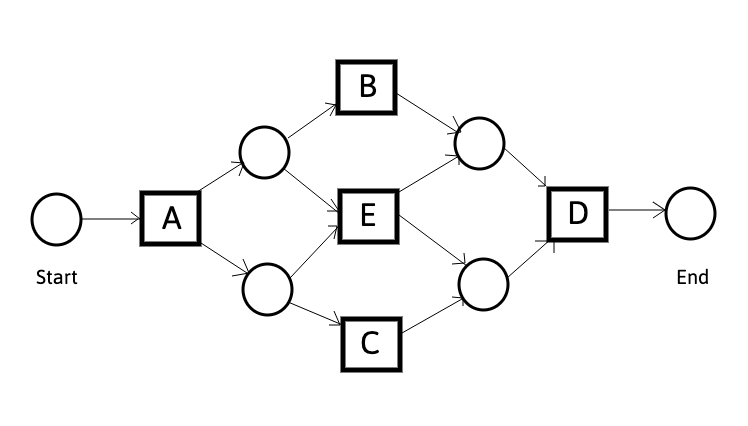
\includegraphics[width=\textwidth,height=\textheight,keepaspectratio]{images/img_alpha_petri_output}\\
\label{fig:example}
\end{center}
\end{figure}

 \newpage

\subsection{Korlátozások}
\begin{itemize}
\item \textbf{Implicit helyek}: Az Alpha bányász nem tud különbséget tenni az implicit és a szükséges helyek között, így a felfedezett petri hálóban előfordulhatnak plusz szükségetelen helyek.
\item \textbf{Ciklusok}: Az Alpha bányász nem képes 1-gyes és 2-tes hosszúságú ciklusok felismerésére a folyamatmodellben.
\item A helyi függőségeket gyakran nem veszi észre az Alpha bányász.
\end{itemize}

\textit{Forrás: \cite{wiki:001}.}\\


\Section{Robotic Process Automation} 
Mi is ez, 
Alkalmazási területek, 
Meglévő rendszerek

\Section{Delphi}
Delphi mint programozási nyelv, 
Miért Delphi a dolgozathoz

